
\chapter{Grundlagen}
\begin{itemize}
	\item im nachfolgenden Erklärungen zu den grundlegenden Konzepten der Arbeit
	\item zunächst werden einfache Kompressionsverfahren angesprochen, welche für die späteren Untersuchungen relevant sind
	\item Danach wird der Fragestellung nachgegangen, warum ein großer Wert auf Sicherheitsmerkmale in Datenbanksystemen gelegt wird
	\item Mit dieser Grundlage wird nun auf Intel SGX eingegangen, die allgemeine Funktionsweise erklärt und ein technischer Überblick gegeben
\end{itemize}
\section{Sicherheit in Datenbanksystemen}
\begin{itemize}
	\item Trusted Computing Base (TCB) %möglicherweise als Definition
	\item Schutzziele
	\subitem Vertraulichkeit
	\subitem Integrität
	\item Zunächst muss Angreifermodell geklärt werden
	\subitem Neugieriger/böswilliger Datenbankadministrator
\end{itemize}
\section{Intel Software Guard Extensions}
\begin{itemize}
	\item erstmals 2013 beschrieben
	\item offiziell unterstützt seit der 6. Generation von Intel Core Prozessoren (Codename Skylake), herausgekommen 2015
\end{itemize}
\section{Kompression von Daten}
\begin{itemize}
	\item In-Memory Datenbanken sind eine große Entwicklung in den letzten Jahren
	\item dabei werden sämtliche Daten im Hauptspeicher gespeichert und verarbeitet, statt im Sekundärspeicher (Festplatte), wo Zugriffszeiten bei weitem größer sind
	\item um den Speicherplatz im Hauptspeicher effektiv zu nutzen, eignen sich schnelle Kompressionsverfahren, welche den Speicherplatz bei der Speicherung und Verarbeitung jener Daten reduzieren
	% TODO Verweis auf Julianas Diplomarbeit!?
	\item diese leichtgewichtigen Kompressionsverfahren sind schneller als schwergewichtige Varianten wie Huffman Kodierung, weisen jedoch keine derart hohen Kompressionsraten auf, da kein Kontextwissen in die Berechnung einfließt, bspw. die Frequenz eines bestimmten Wortes, wie das bei Huffman der Fall ist
	\item Im Folgenden werden zwei jener Verfahren vorgestellt, die auch bei späteren Tests zum Einsatz kommen: VByte und Lauflängenkodierung
	\item Ziel ist es, ein grundlegendes Verständnis für die Funktionsweise der beiden Verfahren zu vermitteln, da diese bei späteren Performancetests eingesetzt werden und in einer Intel SGX Enclave laufengelassen werden
\end{itemize}
\subsection{VByte}
\subsection{Lauflängenkodierung}
\section{Verwandte Arbeiten}
Auf dem Gebiet der sicheren Datenhaltung und -verarbeitung gab es in der Vergangenheit bereits viele vielversprechende Lösungsansätze. In diesem Kapitel wird ein Überblick über entsprechende Arbeiten gegeben. Die größten Vertreter werden zudem etwas genauer auf ihre Vor- und Nachteile untersucht. Hierbei sind die Hauptmerkmale vor allem die zur Verfügung gestellte Sicherheit, unter dem kryptographischen Gesichtspunkt und auch der Möglichkeit zur Anpassbarkeit jener. Darüber hinaus stellt sich auch die Frage, inwieweit die Funktionalität des Datenbanksystems beeinflusst wird. Etwa, ob es eine Einschränkung der Datenbankschnittstelle gibt, z.B. in Bezug auf die zur Verfügung stehenden Anfragen, oder ob starke Kompromisse auf leistungstechnischer Ebene eingegangen werden müssen.

Ein grundlegender Ansatz, den alle betrachteten Arbeiten gemeinsam haben, ist die Auslagerung und Verschlüsselung der zugrundeliegenden Datenbank. Entsprechend findet meist eine klare Trennung zwischen der reinen Datenspeicherung und der Verarbeitung statt, wobei letztere stets eine unabhängig betrachtete Komponente darstellt. Es lassen sich dennoch zwei Kategorien von Ansätzen festmachen. Zum Ersten ist dies ein rein auf dem Verschlüsselungsverfahren beruhendes Prinzip. Die Daten werden hierbei mit einem bestimmten Schema verschlüsselt, so dass weiterhin eine Verarbeitung stattfinden kann, ohne auf eine Repräsentation in Klartext zugreifen zu müssen. Der zweite Ansatz beruht auf die Einbeziehung von vertraulichen Hardwarekomponenten in den Berechnungsprozess. Diese agieren als sogenannte Vertrauensbereiche und erlauben ein Arbeiten auf den Klartextdaten, ohne dass ein potenzieller Angreifer einen Einblick in diese bekommen kann.

Zunächst wird in diesem Kapitel auf Arbeiten aus der ersten Kategorie eingegangen. Der bekannteste Vertreter ist hierbei CryptDB. In seinem Bereich bildet es den Grundstein für die weiteren hier aufgeführten Arbeiten und wird etwas genauer behandelt. Basierend auf Vertrauensbereichen sind sehr vielfältige Arbeiten entstanden. Betrachtet werden hier vor allem TrustedDB, Cipherbase und VC3. Letzteres ist einer der neuesten Entwicklungen und nutzt selbst Intel SGX. In Abbildung \ref{fig:timeline} ist eine einfache zeitliche Einordnung der verschiedenen Arbeiten zu sehen. Für einen besseren Überblick sind Intel SGX und VC3 in einer eigenen Zeitlinie dargestellt.

\begin{figure}
	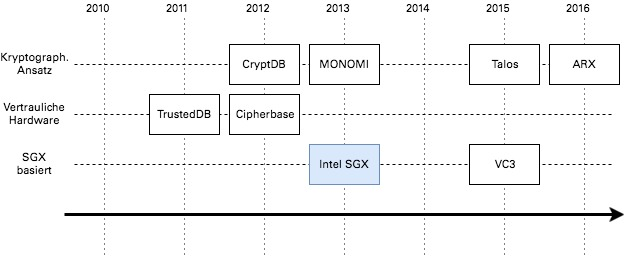
\includegraphics[width=0.9\linewidth]{img/RelatedWorkTimeline.pdf}
	\centering
	\caption{Zeitliche Einordnung verwandter Arbeiten nach Kategorie}
	\label{fig:timeline}
\end{figure}

%TODO subsubsection?
Genau wie die meisten anderen Systeme, wurde CryptDB \cite{Popa2011}\cite{Popa2012} für die Arbeit auf relationalen SQL Datenbanken entworfen. Der Kern von CryptDBs Architektur ist ein Proxy Server, der sich zwischen dem Anwendungs- und  Datenbankserver befindet. Sobald eine Anfrage an die verschlüsselte Datenbank gestellt wird oder eine Antwort zurückkommt, verlaufen diese zunächst über jenen Proxy, der im Normalfall ebenfalls auf dem Anwendungsserver läuft. Ein vereinfachtes Schema der Architektur ist in Abbildung \ref{fig:cryptdb} zu sehen. CryptDB nutzt den Aufbau von SQL Anfragen aus mehreren einfachen Operationen wie Joins, Gleichheitsprüfungen oder Ordnungen auf Werten aus, um diese direkt auf den verschlüsselten Daten durchführen zu können. Das entsprechend eingesetzte Verschlüsselungsschema wird als \textit{SQL aware encryption} bezeichnet. Es definiert die kryptographischen Methoden, welche für die Ausführung einer bestimmten Operation notwendig sind. Ist es beispielsweise nur nötig, eine Selektion mit Gleichheitsbedingung durchzuführen, so genügt ein deterministisches Verschlüsselungsverfahren, welches stets den gleichen Schlüsseltext für einen gegebenen Klartext produziert. Will man allerdings den minimalen oder maximalen Wert, bzw. eine geordnete Ergebnismenge erhalten, so ist es nötig ein schwächeres Verfahren einzusetzen, welche die Ordnung von Klartextwerten durch das Verschlüsseln erhält, sogenannte \textit{Order Preserving Encryption}. Um eine möglichst große SQL Funktionalität bereitzustellen und dennoch das höchstmögliche Maß an Vertraulichkeit, setzt CryptDB auf ein sogenanntes \textit{Onion Scheme}. Jeder Wert ist in mehreren Schichten verschlüsselt, wobei die gegebene Sicherheit mit jeder Schicht zunimmt, ebenso nehmen die möglichen Operationen ab. Entschlüsselt wird dann nur bis zu der Schicht, welche für die aktuellen Berechnungen nötig ist. Die benutzten Schlüssel liegen je Nutzer auf dem Anwendungsserver. Der Proxy selbst besitzt jedoch einen Masterkey, um Anfragen umschreiben zu können. Da jeder Benutzer des Systems über einen individuellen Schlüssel verfügt, ist es möglich, gewisse Daten für einzelne Nutzer freizugeben oder zu verstecken. Hierfür hält der Proxy ein spezielles Schema. Die Datenverarbeitung selbst erfolgt durch UDFs (User Defined Functions) auf dem Datenbankserver, nachdem der Proxy die eingehende Anfrage umgeschrieben hat. Infolge der Auslieferung von den verschlüsselten Ergebnisdaten an den Proxy, kann dieser die Entschlüsselung vornehmen und sie dem Anwendungsserver liefern.

Trotz der zusätzlichen Bearbeitung im Proxy, hat CryptDB einen relativ geringen Performance Overhead im Vergleich zum herkömmlichen unsicheren Ablauf \cite{Popa2012}. Die Nachteile des Verfahrens liegen allerdings in den eingeschränkten Möglichkeiten an SQL Anfragen, sowie den fehlenden Konfigurationsmöglichkeiten in Bezug auf die gewünschte Sicherheit. Die absichtliche Nutzung schwächerer Verschlüsselungsverfahren wie OPE, erleichtern einem Angreifer, Aussagen über die Schlüsseltexte zu treffen \cite{Poddar2016}.

Zwei Jahre nach der Veröffentlichung von CryptDB folgte mit MONOMI \cite{Tu2013} ein nachfolgendes System, welches auf dem Verschlüsselungsschema aufbaute, jedoch für den Anwendungsfall von analytischen Workloads angepasst wurde. Diese unterscheiden sich größtenteils dadurch, dass viel größere Datenmengen auf komplexe Art verarbeitet werden. Dies bringt auf einer komplett verschlüsselten Datenbank viele Probleme mit sich, unter anderem, wie jene komplexen Anfragen effizient auf verschlüsselten Daten ausgeführt werden können. MONOMI verteilt hierzu die Ausführung der Anfragen auf Server und Client. Bei Letzterem können so etwa letzte Verarbeitungsschritte ausgeführt werden, nachdem die Daten schon unverschlüsselt sind, während jene auf dem Server mit den verschlüsselten Daten deutlich aufwendiger wären. MONOMI bringt zudem noch weitere Leistungsoptimierungen mit und schneidet bei großen Benchmarks sowohl in Bezug auf Speicherbedarf und Leistung deutlich besser ab als CryptDB \cite{Tu2013}.

An dieser Stelle muss auch kurz Talos \cite{Shafagh2015} erwähnt werden. Das 2015 beschriebene System baut ebenso auf CryptDB auf, vereinfacht und optimiert das Konzept jedoch für den Einsatz im Internet of Things. Die eingesetzten kryptographischen Algorithmen, z.B. für OPE werden durch leistungsfähigere Varianten ersetzt und erlauben die Ausführung auf Systemen mit beschränktem Energiebudget und Speicherplatz.

Der letzte hier genannte Vertreter in der Kategorie ausschließlich auf Kryptographie beruhender Systeme ist Arx \cite{Poddar2016}. Es handelt sich dabei um einen ganz offiziellen Nachfolger von CryptDB, der 2016 veröffentlicht wurde. Diesmal verfolgte man eine neue Herangehensweise, indem man die Berechnungen nicht auf den eingesetzten Verschlüsselungsverfahren aufsetzt, sondern in spezielle Datenstrukturen. Dies erlaubt es, komplett unabhängig vom Verschlüsselungsverfahren zu sein, was wiederum erlaubt, ausschließlich starke und anerkannte Standardverfahren wie AES zu nutzen. Ermöglicht wird dies durch die Nutzung von speziellen Datenbankindizes, welche speziell zum Traversieren verschlüsselter Daten entworfen wurden und die Sicherheit dahingehend gewähren, dass die Knoten in den Indexstrukturen nach jeder Benutzung zerstört und entsprechend erneuert werden müssen.

\begin{figure}
	\includegraphics[width=0.9\linewidth]{img/RelatedWorkCryptDB.pdf}
	\centering
	\caption{Architektur von CryptDB}
	\label{fig:cryptdb}
\end{figure}

Auf Seiten der Verfahren, welche anstatt der reinen Arbeit auf verschlüsselten Daten vertrauliche Hardwarekomponenten nutzen, soll zunächst TrustedDB \cite{Bajaj2013} behandelt werden. Genau wie CryptDB wurde es 2011 publiziert, wodurch die beiden Vorgehensweisen quasi stets koexistierten. TrustedDB erweitert den üblichen Datenbankserver um die zusätzliche Einbeziehung eines sicheren Koprozessors (SCPU), wie diese zum Beispiel von der Firma IBM hergestellt werden, um eine gesicherte Datenverarbeitung zu gewährleisten. Bei der Definition des Datenbankschemas können einzelne zu schützende Attribute entsprechend ausgezeichnet werden. Anhand von \ref{fig:trusteddb} wird die Funktionsweise des Verfahrens vereinfacht erklärt. 

\begin{figure}[h]
	\includegraphics[width=0.9\linewidth]{img/RelatedWorkTrustedDB.pdf}
	\centering
	\caption{Ablauf einer Datenbankanfrage unter TrustedDB}
	\label{fig:trusteddb}
\end{figure}

Bei einer Anfrage des Clients wird diese zunächst verschlüsselt, bevor sie zum Server gelangt (1). Der unsichere Teil des Servers kann die Anfrage in der Form nicht bearbeiten und leitet sie an die SCPU weiter. Nach der Entschlüsselung findet dort eine Unterteilung in Teilanfragen statt, unter dem Gesichtspunkt, ob diese die Verarbeitung sensibler oder harmloser Daten beinhalten (2). Ergebnis ist folglich eine Menge sogenannter \textit{public} und \textit{private queries}. Erstere kann die herkömmliche Datenbankengine übernehmen (3). Dies ist in der Regel ein deutlich größerer Anteil der Daten. Die SCPU übernimmt nur die private queries, also nur den Teil der Arbeit, für den sie tatsächlich geeignet ist (4). Die Ergebnisse werden zum Schluss zusammengefügt und verschlüsselt zum Client zurückgeschickt (5), der diese wiederum entschlüsselt (6). Als großer Vorteil wird unter anderem die bessere Leistung gegenüber der kryptographischen Berechnungen in Software beschrieben. Zudem gibt es keine Einschränkungen an möglichen SQL Anfragen. Jedoch erfordert TrustedDBs Architektur das Einbetten eines gesamten Datenbanksystems in die SCPU und somit in die Trusted Computing Base. Aufgrund der beschränkten Ressourcen des Koprozessors muss hier zudem auf eine funktionsarme SQLite Datenbank zurückgegriffen werden \cite{Arasu}. Sobald ein größerer Anteil der Daten als sensitiv eingestuft wird und die SCPU somit in größerem Maße beansprucht, so nimmt die Leistung stark ab, da dessen Rechenleistung stark eingeschränkt ist \cite{Arasu2012}.

Im Gegensatz zu TrustedDB setzt Cipherbase \cite{Arasu2012}\cite{Arasu} auf einen sehr eng gekoppelten Ansatz und verspricht somit ein deutlich leistungsfähigeres System. Es erweitert ursprünglich den Microsoft SQL Server um eine \textit{Trusted Machine}. Eine Besonderheit ist die Umsetzung jener als einfache Stackmaschine, auf welcher ausschließlich die Berechnung der kryptographischen Primitive abläuft. Zur Realisierung der Trusted Machine eignen sich zum Beispiel FPGAs \cite{Arasu}. Außerdem kommen die bereits aus CryptDB bekannten Operationen auf verschlüsselten Daten zum Einsatz, jedoch ohne die Nutzung einer schichtweisen Verschlüsselung bei der Datenhaltung, welche es einem Angreifer einfacher macht Informationen zu gewinnen. Um Letzteres zu erreichen setzt man auf ein statisches Modell, wodurch die Daten einmalig mit der benötigten Methode unter Gewährleistung bestimmter Funktionalität, z.B. der Möglichkeit für Bereichsanfragen, verschlüsselt werden. Die freie Konfiguration der benötigten Sicherheit je Spalte ist ein großer Vorteil gegenüber CryptDB. Das enge Hardware Software Codesign erlaubt eine bessere Leistung gegenüber TrustedDB, während die Trusted Computing Base möglichst klein gehalten wird \cite{Arasu}. Zudem gibt es keine Limitierungen in Bezug auf die unterstützte Ausdrucksmächtigkeit von Anfragen, da ein einziges Datenbanksystem von industrieller Stärke erweitert wird \cite{Arasu2013}. Die Preisgabe der Ordnung von Daten unter Nutzung eines ordnungserhaltenden Verschlüsselungsschemas ist aber auch hier als Nachteil zu nennen.

Zuletzt wird mit VC3 (Verifiable Confidential Cloud Computing) \cite{Schuster2015} kurz ein auf Intel SGX basierender Ansatz behandelt. Der konkrete Anwendungsfall ist hierbei die sichere Ausführung von verteilten Berechnungen nach dem \textit{MapReduce} Modell in der Cloud. Jeder Arbeitsknoten führt seine Funktion (\textit{Map} oder \textit{Reduce}) in einer gesicherten Enclave aus, während die Daten zwischen den Knoten stets verschlüsselt vorliegen. Vor Beginn des Verarbeitungsprozesses werden jene Funktionen zunächst als Schlüsseltexte in die Knoten geladen. Zu Beginn eines Jobs laden diese jeweils ein Programm zum sicheren Schlüsselaustausch in die Enclave und führen es aus, um sich mit dem Nutzer auf einen Schlüssel zu einigen. Dieser wird benutzt um die Map und Reduce Funktionen sowie die später ein- und ausgehenden Daten zu entschlüsseln. Der große Vorteil ist in diesem Szenario, dass die Knoten nach außen hin auf herkömmliche Art behandelt werden können, wodurch Mechanismen wie Load Balancing auch weiterhin funktionieren.

%TODO Outro des Kapitels